\documentclass[main.tex]{subfiles}
\begin{document}

环路增益不能无限制地增大,当考虑动态响应时,反馈的高环路增益可能会使系统响应变得更差,甚至引起系统不稳定。如何获得尽可能高的增益而不破坏系统的稳定性,是大多数反馈控制设计所需要考虑的问题。

\section{经典控制原理}
经典控制是基于拉普拉斯变换和傅里叶变换的控制。
\subsubsection{Introduction}
Closed-Loop System 传递函数: 
\begin{equation}
    M(s) = \frac{Y(s)}{R(s)} = \frac{G(s)}{1+G(s)H(s)}
\end{equation}

Open-Loop System 传递函数:
\begin{equation}
    M(s) = G(s)|_{H(s)=0}
\end{equation}

\subsubsection{Mathematical Foundation and Stability}

对于一个最简单的电感、电阻、电容串联电路有:
\begin{equation}
    R\cdot i(t) + L\cdot \frac{di(t)}{dt}+\frac{1}{C}\cdot\int i(t')dt' = e(t)
\end{equation}

Define that:

\begin{equation}
    \begin{aligned}
        x_1(t) &= \int i(t')dt' \\
        x_2(t) &= \frac{dx_1(t)}{dt} = i(t) \\
    \end{aligned}
\end{equation}

$\Longrightarrow$

\begin{equation}
    \begin{aligned}
        Rx_2 + L\dot x_2 + \frac{1}{C}x_1 = e \\
        \dot x_2 = -\frac{1}{LC}x_1 - \frac{R}{L}x_2+\frac{1}{L}e \\
    \end{aligned}
\end{equation}

状态方程(State Equation:矩阵形式的一阶微分方程):

\begin{equation}
    \begin{bmatrix}
    \dot x_1 \\
    \dot x_2 \\
    \end{bmatrix}
    =
    \begin{bmatrix}
        0 & 1 \\
        -\frac{1}{LC} & -\frac{R}{L}
    \end{bmatrix}
    \begin{bmatrix}
        x_1 \\
        x_2 \\
    \end{bmatrix}
    +
    \begin{bmatrix}
        0\\
        \frac{1}{L}\\
    \end{bmatrix}
    e
\end{equation}

\begin{equation}
    x_0 = 
    \begin{bmatrix}
        x_1(0) \\
        x_2(0) \\
    \end{bmatrix}
\end{equation}

输出方程(Output Equation):
The Output of the capacitor:
\begin{equation}
    \begin{aligned}
    y &= v_c(t) = \frac{1}{C} \int i(t')dt' = \frac{1}{C}x_1 \\
    y &= v_c = 
    \begin{bmatrix}
        \frac{1}{C} & 0\\
    \end{bmatrix}
    \begin{bmatrix}
        x_1 \\
        x_2 \\
    \end{bmatrix}
    + 0\cdot e
    \end{aligned}
\end{equation}

拉普拉斯变换的积分区间为实数。收敛域为$Re(s) > 0$,原因如下:

拉普拉斯变换是傅氏变换的一种推广,拉普拉斯变换没有要求要收敛,真正需要收敛的是傅氏变换,傅里叶变换必须满足狄利克雷条件,而不是所有的函数都满足:定义域从-∞延伸到+∞的信号必须要正向和反向在区域无穷时都为0,也就是说正反均要收敛。如果是因果信号,那么只要求正向收敛。定义拉普拉斯变换为$\mathcal{L}(f(t)e^{-at})$,如果$f(t)$发散,那么其乘以一个收敛的指数函数可能会收敛,指数函数的收敛域为a>0,a即为复频率变量s的实部。

所以双边初等函数不存在拉普拉斯变换,因为其必定会一边发散一边收敛或维持常数。拉普拉斯逆变换可用部分分式展开法\\[2pt]

\textbf{Important Theorems of the L.T.}

\begin{enumerate}
    \item $\mathcal{L}[\frac{df}{dt}] = sF(s)-f(0)$
    
    s的物理意义是给系统增加一个零点
    
    In General,

    $\mathcal{L}[\frac{d^nf}{dt^n}]=s^nF(s)-s^{n-1}f(0)-s^{n-2}f^{(1)}(0)-...-f^{(n-1)}(0)$
    
    \begin{example}
    $\frac{s}{s+1}$
    \begin{figure}[H]
        \begin{minipage}{0.5\textwidth}
            \centering
            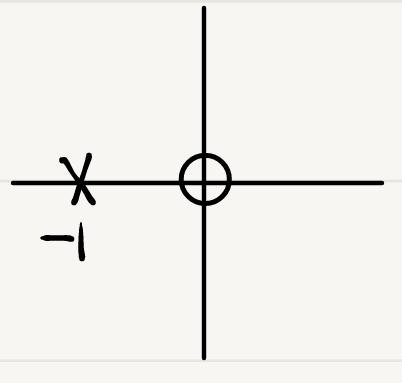
\includegraphics[width=0.36\textwidth]{img/img_2.1.1.png}
        \end{minipage}
        \hfill
        \begin{minipage}{0.4\textwidth}
            $\rightarrow$在原点处有零点代表控制框图里有微分器,滤除所有DC信号
        \end{minipage}
    \end{figure}
    \end{example}
    微分器$\cdot s$后按照频率角度来说,$|sF(s)| = |\omega|\cdot|F(j\omega)|$,会放大高频

    \item $\mathcal{L}[\int^t_0f(\tau)d\tau] = \frac{1}{s}F(s)$
    
    Moreover, $L[n \quad times\quad int] = \frac{F(s)}{s^n}$

    相当于积分器,会放大低频,滤过高频。注意:放置太多pole在原点,可能会导致系统不稳定。

    \item Shift in Time:$\mathcal{L}[f(t-T)u_s(t-T)]=e^{-sT}F(s)$
    \item Initial-Value Theorem: $f(0) = \lim\limits_{s\to\infty}sF(s)$
    \item Final-Value Theorem: $\lim\limits_{t\to\infty} f(t) = \lim\limits_{s\to 0}sF(s)$

    Condition: $sF(s)$在右半平面是有界值,极点没有在右半平面且没有在原点以外的虚轴上
    
    Application: 探究控制系统的稳定性

    \item Complex shift: $L[e^{\alpha t}f(t)] = F(s-\alpha)$   载波

    \item Convolution $\mathcal{L}[f_1(t)\otimes f_2(t)] = F_1(s)F_2(s)$,$L(\mathcal{L}[f_1(t)f_2(t)]) = F_1(s)\otimes F_2(s)$
\end{enumerate}

\textbf{零极点设计}:
\begin{figure}[H]
    \centering
    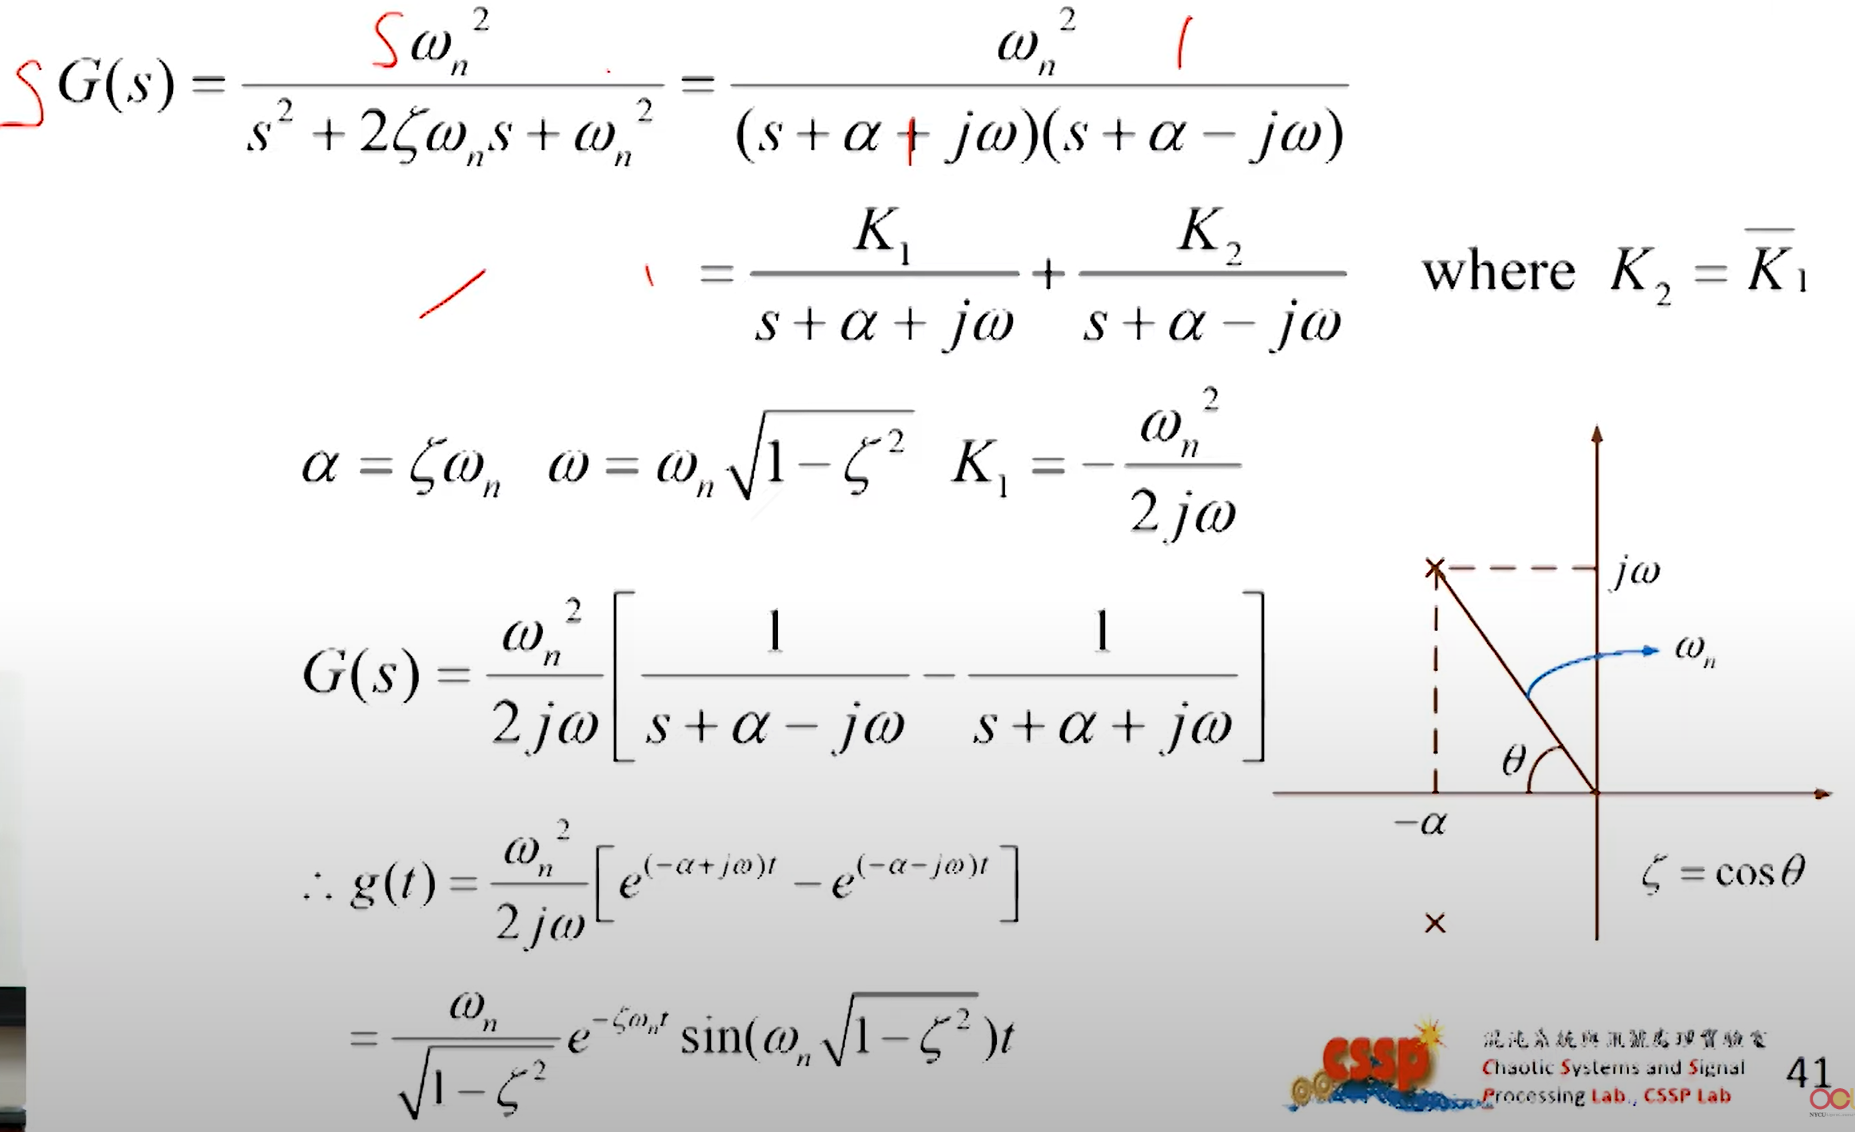
\includegraphics[width=0.8\textwidth]{img/img_2.1.3.png}
    \caption{Complex-Conjugate Poles}
    \label{Complex-Conjugate Poles}
\end{figure}
\begin{figure}[H]
\begin{minipage}{0.5\textwidth}
    \centering
    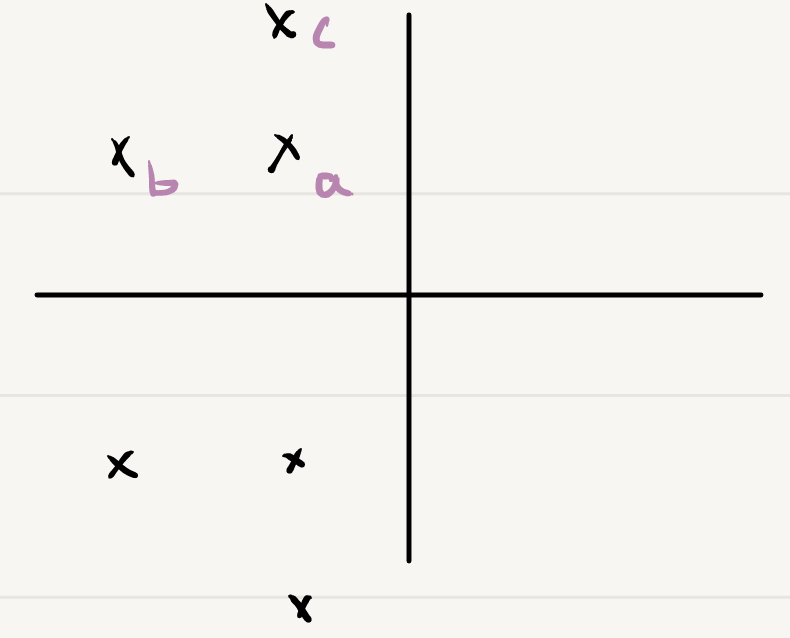
\includegraphics[width=0.5\textwidth]{img/img_2.1.2.png}
    \caption{零极点设计}
    \label{fig:zero-pole design}
\end{minipage}
\hfill
\begin{minipage}{0.5\textwidth}
    ac点比b点收敛慢,c点比ab点震荡大(虚部看震荡,实部看衰减),从原点到各点的距离表示频宽,各点与原点连线与实轴负半轴的夹角叫做$\theta$,$\theta$越大超调量越大
\end{minipage}
\end{figure}

\textbf{Stability: SISO System}
\begin{itemize}
    \item Absolutely stable: stable or not
    \item Relatively stable: how stable
    \item Zero-state response
    \item Zero-input response
    \item Total response = Zero-state response + Zero-input response
\end{itemize}




\end{document}